\chapter{Transition Systems, Access Control, Security, Trust, and
  Logic}
% \label{introduction}
% \chinbox{
%   \begin{itemize}
%   \item Introduce each of the following:
%     \begin{enumerate}[{-}]
%     \item Access control logic
%     \item Structural operational semantics
%     \item ML and HOL
%     \end{enumerate}

%   \end{itemize}
% }

\begin{quote}
  \emph{``Without analysis and synthesis across a variety of domains
    or across a variety of competing/independent channels of
    information, we cannot evolve new repertoires to deal with
    unfamiliar phenomena or unforseen change.''}\hfill{-- John
    R. Boyd, \emph{The Essence of Winning and Losing,} 1995}
\end{quote}

This book is about access control, security, and trust. We wrote this
book for people who specify, design, and verify computer and
information systems that must be trustworthy and secure. Most every
information system or computer has some security requirement.  Common
examples include computers handling sensitive information such as
financial information, health records, or military secrets. If you are
responsible for designing, building, testing, or certifying systems
that have security concerns, then you are concerned with the
following:
\begin{itemize}
\item who or what can access protected resources,
\item how to protect the confidentiality, integrity, and availability
  of those resources,
\item who or what is trusted or believed, and
\item compelling reasons to conclude a system is worthy of trust.
\end{itemize}

For example, if you are responsible for the specification, design, or
operation of computers holding bank accounts, you are very concerned
about the following questions:
\begin{itemize}
\item Who can withdraw funds from a customer's bank account
  electronically?
\item Who is allowed to alter the balance or available funds in a
  customer's account?
\item Who has authority to grant account access?
\item What evidence is there to substantiate that the computerized
  banking system is secure and operating correctly?
\end{itemize}

An oft-quoted and ignored security principle is \emph{security must be
  designed into systems from the start.} Another oft-quoted and
ignored design principle is complete mediation: \emph{every access to
  every object must be checked for authority}, \cite{SS75}. Systems
and designers routinely ignore the above two principles. Thus, the
bedrock of security, knowing who has access to what and under what
circumstances in terms of policies, concepts of operations, and
enforcement mechanisms, is largely missing. This observation is not an
assertion that designers and engineers are malicious or lazy as a
group. Quite the contrary, designers and engineers as a group are
dedicated to building systems correctly and securely. What they lack
are the mathematical and logical tools to help them develop and verify
their thinking and designs.

As an experiment, try to think about something without using words or
language. As another experiment, try describing an algebraic property
or procedure without using mathematical symbols. The point of these
mental experiments is to illustrate the difficulty of describing and
reasoning about concepts without appropriate language, symbols, and
properties.  Security is no different. How can designers be held
accountable for formally verifying access-control policies, concepts
of operations, software, operating systems, and hardware unless they
have the necessary technology in terms of languages, calculi, and
computer-assisted reasoning tools to describe and verify their access
control policies and enforcement mechanisms?

Any engineer or computer scientist who has designed, certified, or
worked with systems of any size or consequence knows that a key
question is \emph{how will we know?}  They know that undetected design
flaws or inappropriate assumptions that are built into deployed
systems are potentially disastrous and life threatening. They know
that flaws in deployed systems are orders of magnitude more costly to
remedy when compared to corrections made in the design phase. They
know that undetected flaws potentially destroy systems, destroy
reputations, and destroy credibility, leading to failed missions,
failed services, and failed corporations.  In short, as systems become
larger and more complex, it is increasingly difficult for designers
and certifiers to get a good night's sleep.

Our purpose in writing this book is to help designers and certifiers
sleep well at night.  Our experience shows us that the system designers
and certifiers who sleep best at night are those who combine their
experience and intuition with mathematics and logic.  Experience and
intuition are powerful tools that inform the selection of a design
approach. Mathematics and logic are unparalleled in providing
assurances of correct coverage of all cases and instances, some of
which might not have been imagined by designers or certifiers.

We follow the same approach used by civil, mechanical, and electrical
engineers. Mathematics and logic properly used clarify the underlying
principles and properties of systems. Systems with mathematical and
logical descriptions are amenable to independent and automated
verification and testing. The effects of system changes or
consequences of altering assumptions are easier to deduce with logic
than without.

Our experience shows us that flaws and misconceptions often exist
\emph{between} levels of abstraction in systems.  For example, how
will we know that a security policy related to information integrity
is correctly implemented by hardware and software together?
Requirement writers, software engineers, and hardware engineers might
interpret the meaning of integrity differently leading to improper
assumptions, flawed policies, flawed designs, and failed systems. Our
approach to dealing with this observation is to use a logic that spans
many levels of abstraction including hardware, software, and
policy.

\section{A Logic for Access Control, Security, and Trust}
\label{sec:acl-language}

\section{Reasoning about Transition Systems}
\label{sec:transition-systems}

\section{Theorem Provers}
\label{sec:theorem-provers}

\section{Proof and Uncertainty}
\label{sec:proof-uncertainty}


\begin{figure}[tb]
  \centering
  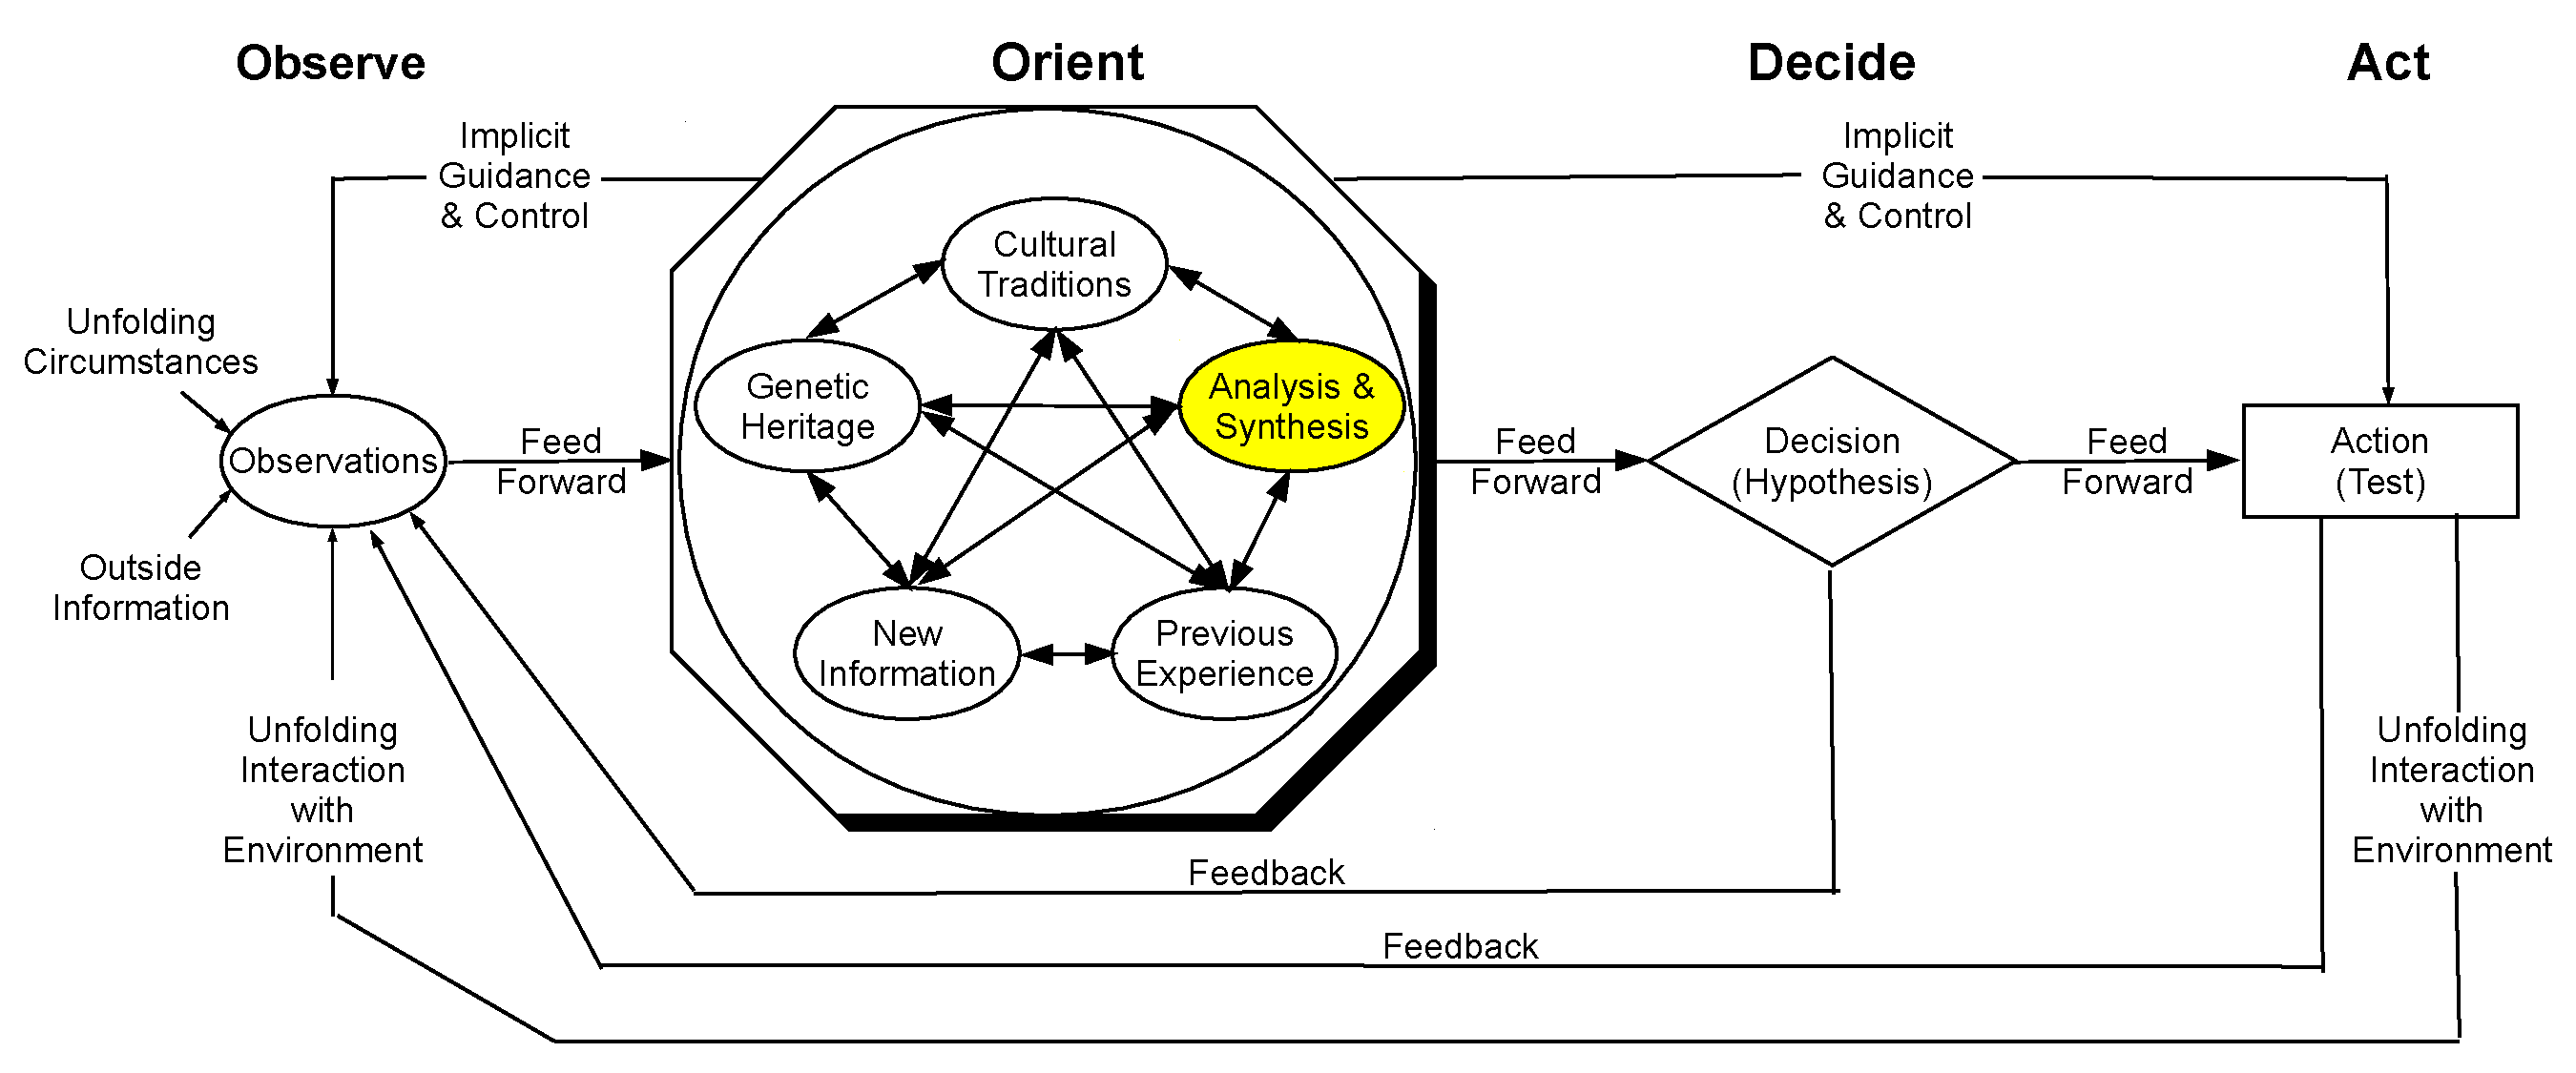
\includegraphics[width=0.9\linewidth]{Figures/Introduction/OODA}
  \caption{John Boyd's OODA Loop}
  \label{fig:ooda-loop}
\end{figure}

\begin{figure}[tb]
  \centering
  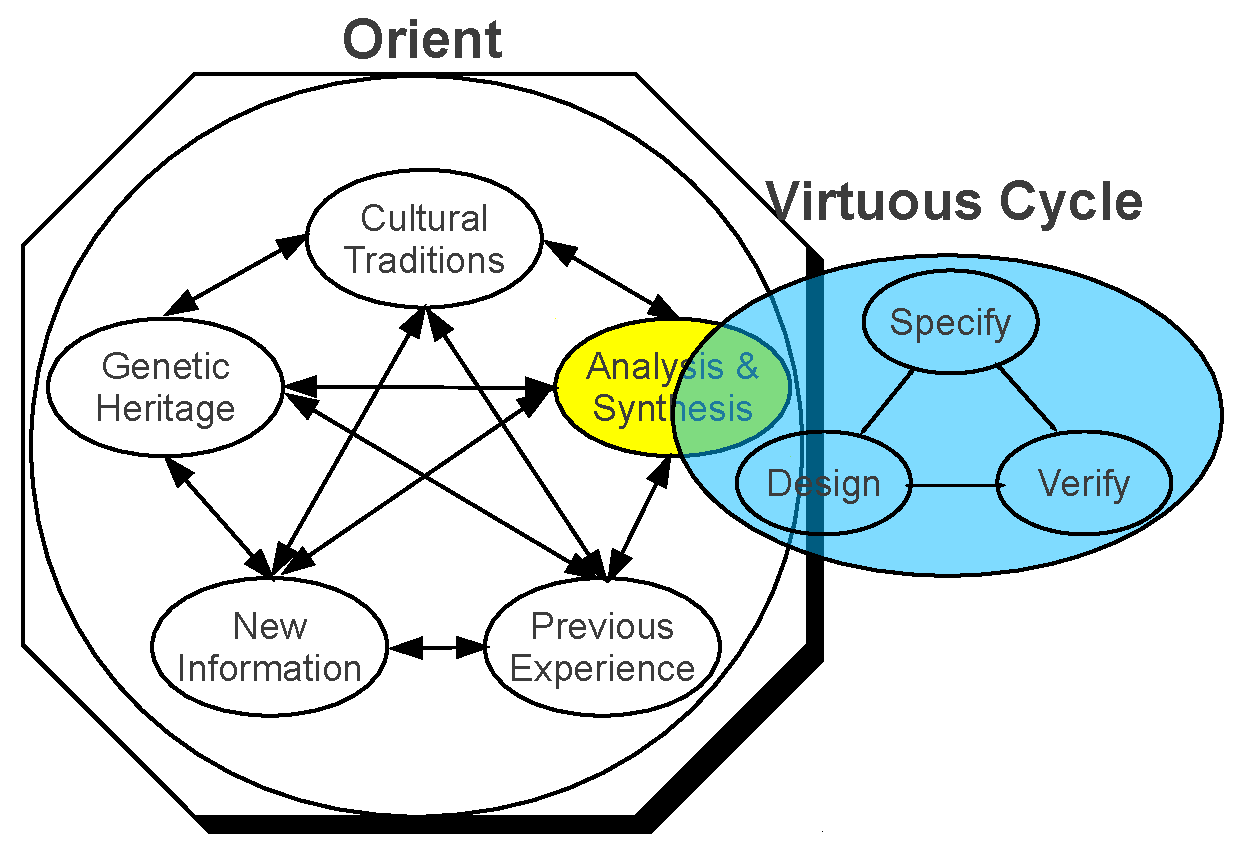
\includegraphics[width=0.6\linewidth]{Figures/Introduction/OrientVirtuousCycle}
  \caption{Orientation and the Virtuous Cycle}
  \label{fig:orient-virtuous-cycle}
\end{figure}
% ---- this points LaTeX to book.tex ---- 
% Local Variables: 
% TeX-master: "book"
% End:

